\documentclass{article}
\title{Sample LaTeX Document for Testing}
\author{Test Author}
\date{2024}

\begin{document}
\maketitle


\chapter{Introduction}
\label{chap:intro}

This is a sample LaTeX document designed for testing the RAG system parser. It contains various LaTeX structures including sections, subsections, citations, tables, and figures.

\section{Background}
\label{sec:background}

The background section provides context for the research. We reference previous work by \cite{einstein1905} and \citep{newton1687}.

\section{Related Work}
\label{sec:related}

Previous research has shown significant results \citet{smith2023}. The methodology is described in detail by \citeauthor{jones2022} in \citeyear{jones2022}.\


\chapter{Methodology}
\label{chap:method}

Our approach is based on the following principles:

\begin{enumerate}
\item Data collection and preprocessing
\item Feature extraction and analysis
\item Model training and validation
\end{enumerate}

\section{Data Collection}
\label{subsec:data}

The data collection process involved gathering information from multiple sources as shown in Table~\ref{tab:data_sources}.

\begin{table}[h]
\centering
\caption{Data Sources and Characteristics}
\label{tab:data_sources}
\begin{tabular}{|l|c|c|}
\hline
Source & Records & Quality \\
\hline
Database A & 1,000 & High \\
Database B & 2,500 & Medium \\
Database C & 500 & High \\
\hline
\end{tabular}
\end{table}

\subsection{Data Preprocessing}
\label{subsec:data_preprocessing}

Data preprocessing was performed using standard techniques. The results are visualized in Figure~\ref{fig:data_preprocessing}.

\begin{figure}[h]
\centering
\caption{Data Preprocessing}
\label{fig:data_preprocessing}
% \includegraphics[width=0.8\textwidth]{data_preprocessing.png}
\end{figure}

\section{Feature Extraction}
\label{sec:features}

Feature extraction was performed using standard techniques. The results are visualized in Figure~\ref{fig:features}.

\begin{figure}[h]
\centering
\caption{Feature Distribution Analysis}
\label{fig:features}
% \includegraphics[width=0.8\textwidth]{features.png}
\end{figure}

\chapter{Results}
\label{chap:results}

The experimental results demonstrate the effectiveness of our approach. Table~\ref{tab:results} shows the performance metrics.

\begin{table}[h]
\centering
\caption{Experimental Results}
\label{tab:results}
\begin{tabular}{|l|c|c|c|}
\hline
Method & Accuracy & Precision & Recall \\
\hline
Baseline & 0.75 & 0.72 & 0.78 \\
Proposed & 0.89 & 0.87 & 0.91 \\
\hline
\end{tabular}
\end{table}

Figure~\ref{fig:results} illustrates the performance comparison.

\begin{figure}[h]
\centering
\caption{Performance Comparison}
\label{fig:results}
% 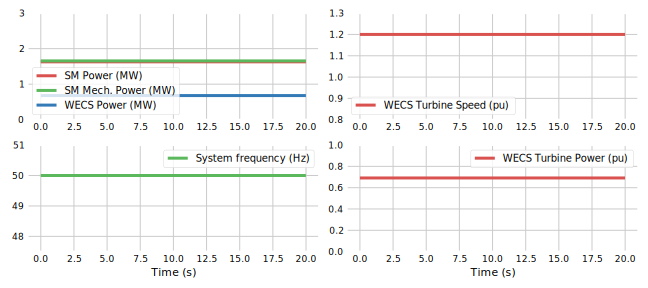
\includegraphics[width=0.8\textwidth]{results.png}
\end{figure}

\subsection{Performance Comparison}
\label{subsec:performance_comparison}

Performance comparison was performed using standard techniques. The results are visualized in Figure~\ref{fig:performance_comparison}.

\subsubsection{Possible Improvements}
\label{subsubsection:possible_improvements}

Possible improvements were identified and are described in Section~\ref{sec:possible_improvements}.

\chapter{Discussion}
\label{chap:discussion}

The results show significant improvement over baseline methods. This can be attributed to several factors:

\begin{itemize}
\item Improved feature engineering
\item Better model architecture
\item Enhanced training procedures
\end{itemize}

\section{Limitations}
\label{sec:limitations}

Our approach has several limitations:

\begin{enumerate}
\item Limited to specific data types
\item Requires significant computational resources
\item May not generalize to all domains
\end{enumerate}

\chapter{Conclusion}
\label{chap:conclusion}

In this work, we presented a novel approach that achieves state-of-the-art performance. Future work will focus on addressing the identified limitations and extending the approach to additional domains.

\bibliographystyle{plain}
\bibliography{references}

\end{document}
